\documentclass[10pt,a4paper]{article}

\usepackage{courier}
\usepackage{filecontents}
\usepackage[T1]{fontenc}
\usepackage{fullpage}
\usepackage[top=1in]{geometry}
\usepackage{graphicx}
\usepackage{listings}
\usepackage{parskip}
\usepackage{verbatim}
\usepackage{textcomp}
\usepackage{url}
\usepackage[usenames,dvipsnames,svgnames,table]{xcolor}
\usepackage{amsmath}  % newly added package
\usepackage{algorithm} % newly added package
\usepackage{algorithmic} % newly added package
\usepackage{amsfonts}
\usepackage{amssymb}
\usepackage{longtable}
%\usepackage{dsfont}   % newly added package
\usepackage{booktabs}

\usepackage{float}
\usepackage{graphicx}
\usepackage{caption}
%\usepackage{subcaption}
\usepackage{multirow}
\usepackage{upquote}
\usepackage{subfloat}
\usepackage{subfigure}


\newenvironment{mysplit}%
  {\arraycolsep 0pt \begin{array}{l}}%
  {\end{array}}

\DeclareMathOperator{\val}{=}  % for p=v atoms
\DeclareMathOperator{\notval}{\neq}  % for p=v atoms

\def\processSimpleFluent{\texttt{\small processSimpleFluent}}
\def\processSDFluent{\texttt{\small processSDFluent}}

\def\happensAt{\texttt{\small happensAt}}
\def\happensAtEv{\texttt{\small happensAtEv}}
\def\happensAtIE{\texttt{\small happensAtIE}}
\def\happensAtProcessed{\texttt{\small happensAtProcessed}}
\def\initially{\texttt{\small initially}}
\def\holdsAt{\texttt{\small holdsAt}}
\def\holdsAtSDFluent{\texttt{\small holdsAtSDFluent}}
\def\holdsAtProcessedIE{\texttt{\small holdsAtProcessedIE}}
\def\holdsAtProcessedSDFluent{\texttt{\small holdsAtProcessedSDFluent}}
\def\holdsAtProcessedSimpleFluent{\texttt{\small holdsAtProcessedSimpleFluent}}
\def\holdsFor{\texttt{\small holdsFor}}
\def\holdsForSDFluent{\texttt{\small holdsForSDFluent}}
\def\holdsForSimpleFluent{\texttt{\small holdsForSimpleFluent}}
\def\holdsForProcessedIE{\texttt{\small holdsForProcessedIE}}
\def\holdsForProcessedSDFluent{\texttt{\small holdsForProcessedSDFluent}}
\def\holdsForProcessedSimpleFluent{\texttt{\small holdsForProcessedSimpleFluent}}
\def\initiatedAt{\texttt{\small initiatedAt}}
\def\terminatedAt{\texttt{\small terminatedAt}}
\def\broken{\texttt{\small broken}}
\def\startE{\texttt{\small start}}
\def\endE{\texttt{\small end}}

\def\simpleFPList{\texttt{\small simpleFPList}}
\def\sdFPList{\texttt{\small sdFPList}}

\def\unionall{\texttt{\small union\_all}}
\def\isetunion{\texttt{\small union}}
\def\intersectall{\texttt{\small intersect\_all}}
\def\isetintersection{\texttt{\small intersection}}
\def\complementall{\texttt{\small relative\_complement\_all}}
\def\abscomplementall{\texttt{\small complement\_all}}
\def\isetdifference{\texttt{\small relative\_complement}}

\def\nbf{\texttt{\small not}}
\def\true{\texttt{\small true}}
\def\false{\texttt{\small false}}
\def\since{\texttt{\small since}}

%------- for complexity formulas

\def\m#1#2{m(#1,#2)}
% \def\m#1#2{m_{#1,#2}}   % ALEX



% --- ugly internals for language definition ---
%
\makeatletter

% initialisation of user macros
\newcommand\PrologPredicateStyle{}
\newcommand\PrologVarStyle{}
\newcommand\PrologAnonymVarStyle{}
\newcommand\PrologAtomStyle{}
\newcommand\PrologOtherStyle{}
\newcommand\PrologCommentStyle{}

% useful switches (to keep track of context)
\newif\ifpredicate@prolog@
\newif\ifwithinparens@prolog@

% save definition of underscore for test
\lst@SaveOutputDef{`_}\underscore@prolog

% local variables
\newcount\currentchar@prolog

\newcommand\@testChar@prolog%
{%
  % if we're in processing mode...
  \ifnum\lst@mode=\lst@Pmode%
    \detectTypeAndHighlight@prolog%
  \else
    % ... or within parentheses
    \ifwithinparens@prolog@%
      \detectTypeAndHighlight@prolog%
    \fi
  \fi
  % Some housekeeping...
  \global\predicate@prolog@false%
}

% helper macros
\newcommand\detectTypeAndHighlight@prolog
{%
  % First, assume that we have an atom.
  \def\lst@thestyle{\PrologAtomStyle}%
  % Test whether we have a predicate and modify the style accordingly.
  \ifpredicate@prolog@%
    \def\lst@thestyle{\PrologPredicateStyle}%
  \else
    % Test whether we have a predicate and modify the style accordingly.
    \expandafter\splitfirstchar@prolog\expandafter{\the\lst@token}%
    % Check whether the identifier starts by an underscore.
    \expandafter\ifx\@testChar@prolog\underscore@prolog%
      % Check whether the identifier is '_' (anonymous variable)
      \ifnum\lst@length=1%
        \let\lst@thestyle\PrologAnonymVarStyle%
      \else
        \let\lst@thestyle\PrologVarStyle%
      \fi
    \else
      % Check whether the identifier starts by a capital letter.
      \currentchar@prolog=65
      \loop
        \expandafter\ifnum\expandafter`\@testChar@prolog=\currentchar@prolog%
          \let\lst@thestyle\PrologVarStyle%
          \let\iterate\relax
        \fi
        \advance \currentchar@prolog by 1
        \unless\ifnum\currentchar@prolog>90
      \repeat
    \fi
  \fi
}
\newcommand\splitfirstchar@prolog{}
\def\splitfirstchar@prolog#1{\@splitfirstchar@prolog#1\relax}
\newcommand\@splitfirstchar@prolog{}
\def\@splitfirstchar@prolog#1#2\relax{\def\@testChar@prolog{#1}}

% helper macro for () delimiters
\def\beginlstdelim#1#2%
{%
  \def\endlstdelim{\PrologOtherStyle #2\egroup}%
  {\PrologOtherStyle #1}%
  \global\predicate@prolog@false%
  \withinparens@prolog@true%
  \bgroup\aftergroup\endlstdelim%
}

% language name
\newcommand\lang@prolog{Prolog-pretty}
% ``normalised'' language name
\expandafter\lst@NormedDef\expandafter\normlang@prolog%
  \expandafter{\lang@prolog}

% language definition
\expandafter\expandafter\expandafter\lstdefinelanguage\expandafter%
{\lang@prolog}
{%
  language            = Prolog,
  keywords            = {},      % reset all preset keywords
  showstringspaces    = false,
  alsoletter          = (,
  moredelim           = **[is][\beginlstdelim{(}{)}]{(}{)},
  MoreSelectCharTable =
    \lst@DefSaveDef{`(}\opparen@prolog{\global\predicate@prolog@true\opparen@prolog},
}

\newcommand{\textttsmall}[1]{\texttt{\small #1}}

% Hooking into listings to test each ``identifier''
\newcommand\@ddedToOutput@prolog\relax
\lst@AddToHook{Output}{\@ddedToOutput@prolog}

\lst@AddToHook{PreInit}
{%
  \ifx\lst@language\normlang@prolog%
    \let\@ddedToOutput@prolog\@testChar@prolog%
  \fi
}

\lst@AddToHook{DeInit}{\renewcommand\@ddedToOutput@prolog{}}

\makeatother
%
% --- end of ugly internals ---


% --- definition of a custom style similar to that of Pygments ---
% custom colors
\definecolor{PrologPredicate}	{RGB}{000, 031, 255}
\definecolor{PrologVar}      	{RGB}{127, 000, 127}
\definecolor{PrologAtom}     	{RGB}{255, 000, 000}
\definecolor{PrologComment}	{RGB}{000, 154, 000}
\definecolor{BackgroundColor}	{RGB}{240, 240, 240}

% redefinition of user macros for Prolog style
\renewcommand\PrologPredicateStyle{\color{PrologPredicate}}
\renewcommand\PrologVarStyle{\color{PrologVar}}
\renewcommand\PrologAnonymVarStyle{\color{PrologVar}}
\renewcommand\PrologAtomStyle{\color{PrologAtom}}
\renewcommand\PrologCommentStyle{\itshape\color{PrologComment}}

% custom style definition 
\lstdefinestyle{Prolog-cvlas}
{
	language		= Prolog-pretty,
	upquote		= true,
	stringstyle	= \PrologAtomStyle
}

% global settings
\lstset
{
	captionpos		= below,
	commentstyle		= \color{PrologComment},	% comment style
	numbers			= left,        				% where to put the line-numbers; possible values are (none, left, right)
%	stepnumber		= 2,						% the step between two line-numbers. If it's 1, each line will be numbered
	numberstyle		= \ttfamily\small,			% the style that is used for the line-numbers
	backgroundcolor	= \color{BackgroundColor},
	frame      		= none,
	columns    		= fullflexible,
	basicstyle 		= \ttfamily\small,
}

\title{Event Calculus for Run-Time reasoning (RTEC):\\ A Manual}

\author{Alexander Artikis and Christos Vlassopoulos \bigskip \\ 
Institute of Informatics \& Telecommunications,\\ NCSR ``Demokritos'',\\ Complex Event Recognition group\\ \url{cer.iit.demokritos.gr}}

\begin{document}

\maketitle
\sloppy

\section{Introduction}

The Event Calculus for Run-Time reasoning (RTEC) is an open-source, logic programming implementation of the Event Calculus \cite{DBLP:journals/ngc/KowalskiS86}, optimised for computing continuous queries on data streams \cite{DBLP:journals/tkde/ArtikisSP15}. RTEC has been successfully used for \emph{composite event recognition}  (`event pattern matching') in various real-world application domains. Composite event (CE) recognition systems accept as input a stream of time-stamped simple, derived events (SDE)s. A SDE is the result of applying a computational derivation process to some other event, such as an event coming from a sensor \cite{EPTSglossary}. Using SDEs as input, event recognition systems identify CEs of interest---collections of events that satisfy some pattern. The `definition' of a CE  imposes temporal and, possibly, atemporal constraints on its subevents, i.e.~SDEs or other CEs. 
Below are a few CE recognition applications in which RTEC has been used:
%
\begin{itemize}
	\item Activity recognition (see \cite{DBLP:journals/tkde/ArtikisSP15} and \url{http://cer.iit.demokritos.gr/cerar}).
	\item City transport \& traffic management  \cite{DBLP:journals/tkde/ArtikisSP15, DBLP:conf/bigdataconf/ArtikisWGKG13, DBLP:conf/edbt/ArtikisWSBLPBMKMGMGK14}.
	\item Maritime monitoring (see \cite{DBLP:conf/debs/PitsikalisADRCJ19, DBLP:conf/edbt/PatroumpasAKVTP15} and \url{http://cer.iit.demokritos.gr/cermm}).
	\item Fleet management (see \cite{DBLP:journals/tplp/TsilionisKNDA19} \url{http://cer.iit.demokritos.gr/cerfm}).
\end{itemize}


The novelty of RTEC lies in the following implementation techniques:

\begin{enumerate}
	\item\textit{Caching}, that helps in avoiding unnecessary re-computations.
	\item\textit{Interval manipulation}, that helps in expressing succinctly complex temporal phenomena.
	\item\textit{Indexing}, that makes RTEC robust to data streams that are irrelevant to the queries we want to compute.
	\item\textit{Windowing}, that supports real-time query computation.
\end{enumerate}


\subsection{Software requirements \& installation}

RTEC is cross-platform. The only software requirement is a Prolog implementation. RTEC has been tested under YAP\footnote{\url{https://en.wikipedia.org/wiki/YAP_(Prolog)}} and SWI\footnote{\url{https://www.swi-prolog.org/}} Prolog, operating in Ubuntu Linux. 

In this manual, we will illustrate the use of RTEC in YAP.

To use RTEC, simply download it from \url{https://github.com/aartikis/RTEC}.





\subsection{A simple example}\label{sec:aSimpleExample}  

We begin with a simple example briefly illustrating  the functionality of RTEC. In the following sections we will have a closer look at the expressivity and reasoning algorithms of RTEC.

Suppose that Chris is having an all but ordinary day. He goes to work in the morning and in the afternoon he finds out that he has won the lottery. In the evening he goes to the pub, but loses his wallet. Ultimately, he goes home at night. We want to know whether Chris is happy or not, as these actions take place. Our story has three events, ``go\_to'', ``lose\_wallet'' and ``win\_lottery'', and three properties, ``happy'', ``location'' and ``rich''. The basic concept of RTEC lies in events taking place and modifying the values of the properties. In the RTEC terminology, these properties are called ``fluents''.

We would like to specify the conditions that make Chris happy in our tiny world. Being rich is such a condition. Another condition could be being at the pub. Therefore, the `union' of these two conditions can meet the needs of a happy man in our example. Winning the lottery makes someone rich. For the sake of the example, let's assume that losing your wallet causes you to stop being rich. 

Now that we have designed the rules that describe our example, we are ready to express them into the logic programming language of RTEC. Use a text editor and create a new file, say  ``\textttsmall{toy\_rules.prolog}'', and paste the following:

\begin{minipage}{\linewidth}
\lstinputlisting[
  style      = Prolog-cvlas,
  caption    = {Event description in RTEC.},
  label	     = {lst:rules}
]{listings/toy_rules.prolog}
\end{minipage}

Following Prolog's convention, variables start with an upper-case letter, while predicates and constants start with a lower-case letter. To test the formalization above, create a new file, ``\textttsmall{toy\_declarations.prolog}'', containing the following:

\lstinputlisting[
	style	= Prolog-cvlas,
	caption	= {Event and fluent declarations.},
	label	= {lst:declarations}
]{listings/toy_declarations.prolog}

The above \emph{declarations} file is a companion to the rules file. It contains information about all the events and fluents of our scenario. In the following section, we will describe the declarations language in detail.

At this point, we need to compile the rules and declarations. To do this, open a terminal, go to the \textttsmall{RTEC/} directory, invoke Prolog and execute the following query:

{\small
\begin{verbatim}
   ?- compileEventDescription('toy_declarations.prolog',
                     'toy_rules.prolog', 'toy_rules_compiled.prolog').
\end{verbatim}
}

If Prolog responds with a message ending in ``yes'' or ``true'' (depending on your Prolog implementation), compilation was successful. During compilation, a new file ``\textttsmall{toy\_rules\_compiled.prolog}'' has been created. This file combines the information provided in the rules and declarations files and is in a form ready for use by RTEC. 

At the next step, we must provide the domain of each variable. Create another file, say ``\textttsmall{toy\_var\_domain.prolog}'', and put the following code in it:

\begin{minipage}{\linewidth}
\lstinputlisting[
  style      = Prolog-cvlas,
  caption    = {Variable domain.}
]{listings/toy_var_domain.prolog}
\end{minipage}

The contents of this file are used for \emph{output entity} (e.g.~fluent) grounding (see Listing \ref{lst:declarations}, lines 49-53). 
Finally, to test our event description, we need an event narrative, such as the following:

\begin{minipage}{\linewidth}
\lstinputlisting[
	style	= Prolog-cvlas,
	caption	= {Event narrative.},
	label	= {lst:stream}
]{listings/toy_event_stream.prolog}
\end{minipage}

%``\texttt{toy\_Event\_stream.prolog}''

We make a series of assertions about what happens at each time in our scenario. \textttsmall{happensAtIE} is a compiled version of the \textttsmall{happensAt} predicate that expresses event occurrences. At 9:00 Chris goes to work. Then, at 13:00 he finds out that he has won the lottery. Subsequently, at 17:00 he goes to the pub. Afterwards, at 19:00 he loses his wallet, and finally at 21:00 he returns home. We group these assertions under the auxiliary \textttsmall{updateSDE} predicate, so that whenever we want to load this narrative we simply call this predicate.

Now we have all the necessary components for narrative assimilation---in this example, the computation of the maximal intervals of the fluents. We simply need to combine the aforementioned files and start the RTEC engine. This may be done by creating a Prolog script, ``\textttsmall{toy\_queries.prolog}'' that contains the following:

\begin{minipage}{\linewidth}
\lstinputlisting[
	style	= Prolog-cvlas,
	caption	= {Narrative assimilation script.},
	label	= {lst:queries}
]{listings/toy_queries.prolog}
\end{minipage}

The code of Listing \ref{lst:queries} accumulates the information contained in the files described above, and combines it with the main file of RTEC, namely ``RTEC.prolog''. Then, we define a predicate ``\textttsmall{performER}''  to automate narrative assimilation. At first we initialize RTEC, by setting four parameters. First, we state that the input facts are temporally sorted. 
%Second, we state that there is no need for `dynamic grounding' --- details about this feature will be presented later.
Second, we state that our input data does not require some form of preprocessing. Finally, the last parameter is the distance between two consecutive timepoints in our dataset, which is 1 time unit. Subsequently, we load the event narrative using the ``\textttsmall{updateSDE}'' predicate we created in Listing \ref{lst:stream}, and finally we call the built-in \textttsmall{eventRecognition} predicate of RTEC for narrative assimilation. We provide two parameters, the current time of the query and how deep in the past will RTEC look for events and fluents in order to calculate the composite events of interest. Here, since we have a small dataset that ends at timepoint 21, we perform one query at time 21 and we take into account account all the input events that took place within the last 21 timepoints, i.e. from the beginning.

Back to Prolog now. Halt any open session with Prolog and start a new one. Then load the Prolog script:

{\small
\begin{verbatim}
   ?- ['toy_queries.prolog'].
\end{verbatim}
}

Again, if Prolog responds with a message ending in ``yes'' or ``true'', then the file loading was successful. We are now ready for narrative assimilation, by typing the command

{\small
\begin{verbatim}
   ?- performER.
\end{verbatim}
}

If Prolog answers ``yes'' or ``true'', that means RTEC has finished the computation of the maximal intervals of fluents. Now we can ask RTEC anything about the processed fluents. For instance, if we want to see when Chris is happy, typing ``\textttsmall{holdsFor(happy(chris)=true,I).}'' will give us the answer:

{\small
\begin{verbatim}
I = [(14,22)]
\end{verbatim}
}

This means that Chris is happy from time 14, right after he won the lottery, until time 22 (not included), when he leaves the pub. A term of the form \textttsmall{(Ts, Te)} in RTEC represents the closed-open interval $\mathit{[T_s, T_e)}$. According to our example, one is happy if he is rich or at the pub. Thus, this answer seems reasonable.

To see the maximal intervals of all fluent-value pairs that have been computed by RTEC, simply type ``\textttsmall{holdsFor(F,I).}'' and press ENTER. You will receive an output that looks like this:

{\small
\begin{verbatim}
F = (location(chris)=home),
I = [(22,inf)] ? ;
F = (location(chris)=pub),
I = [(18,22)] ? ;
F = (location(chris)=work),
I = [(10,18)] ? ;
F = (rich(chris)=true),
I = [(14,20)] ? ;
F = (rich(chris)=false),
I = [] ? ;
F = (happy(chris)=true),
I = [(14,22)] ? ;
F = (happy(chris)=false),
I = []
\end{verbatim}
}

In addition, we can ask what was true at a specific time-point. For instance if we ask ``\textttsmall{holdsAt(F,16).}'' we will find out what was the situation like at time-point 16. RTEC will respond:

{\small
\begin{verbatim}
F = (location(chris)=work) ? ;
F = (rich(chris)=true) ? ;
F = (happy(chris)=true)
\end{verbatim}
}

So, RTEC says that at time-point 16 Chris is at work, rich, and happy.

Now that we have given a brief illustration of the basic functionality of RTEC, we can take a closer look at its language and reasoning techniques.

\section{The RTEC language}\label{sec:RTEC-language}

The time model in RTEC is linear and includes integer time-points. Where \textttsmall{F} is a \emph{fluent}---a property that is allowed to have different values at different points in time---the term \textttsmall{F=V} denotes that fluent \textttsmall{F} has value \textttsmall{V}. Boolean fluents are a special case in which the possible values are \true\ and \false. \textttsmall{holdsAt(F=V, T)} represents that fluent \textttsmall{F} has value \textttsmall{V} at a particular time-point \textttsmall{T}. \textttsmall{holdsFor(F=V, I)} represents that \textttsmall{I} is the list of the maximal intervals for which \textttsmall{F=V} holds continuously. \holdsAt\ and \holdsFor\ are defined in such a way that, for any fluent \textttsmall{F}, \textttsmall{holdsAt(F=V, T)} if and only if \textttsmall{T} belongs to one of the maximal intervals of \textttsmall{I} for which \textttsmall{holdsFor(F=V, I)}. 

An \emph{event description} in RTEC includes rules that define the event instances with the use of the \happensAt\ predicate, the effects of events with the use of the \initiatedAt\ and \terminatedAt\ predicates, and the values of the fluents with the use of the \holdsAt\ and \holdsFor\ predicates, as well as other, possibly atemporal, constraints. Table~\ref{tbl:ec} summarises the RTEC predicates available to the event description developer. 

Fluents are either simple or statically determined. In brief, simple fluents are defined by means of \initiatedAt\ and \terminatedAt\ rules, while statically determined fluents are defined by means of application-dependent \holdsFor\ rules. More details on this distinction will be given shortly.

An event description is a (locally) stratified logic program \cite{local-strat}.
We restrict attention to \emph{hierarchical} event descriptions, those where it is possible to define a function \emph{level} that maps all fluent-values \textttsmall{F=V} and all events to the non-negative integers as follows. 
Events and statically determined fluent-values \textttsmall{F=V} of level $0$ are those whose  definitions do not depend on any other events or fluents. These represent the \emph{input entities}. There are no fluent-values \textttsmall{F=V} of simple fluents \textttsmall{F} in level $0$. 
Events and simple fluent-values of level $n$ ($n>0$) are defined in terms of at least one event or fluent-value of level $n{-}1$ and a possibly empty set of events and fluent-values from levels lower than $n{-}1$. Statically determined fluent-values of level $n$ are defined in terms of at least one fluent-value of level $n{-}1$ and a possibly empty set of fluent-values from levels lower than $n{-}1$. 
Events and fluent-values of level $n$ are the \emph{output entities}.
%Note that fluent-values $F\val V_i$ and $F\val V_j$ for $V_i{\neq}V_j$ could be mapped to different levels. For simplicity however, and without loss of generality, a fluent $F$ itself is either simple or statically determined but not both. 

In the following sections we present in more detail the building blocks of RTEC.

\begin{table}[t]
\caption{Main predicates of RTEC.}\vspace{-.3cm}\label{tbl:ec}
\begin{center}
\renewcommand{\arraystretch}{0.9}
\setlength\tabcolsep{3.8pt}
\begin{tabular}{ll}
\hline\noalign{\smallskip}
\multicolumn{1}{c}{\textbf{Predicate}} & \multicolumn{1}{c}{\textbf{Meaning}}  \\
\noalign{\smallskip}
\hline
\noalign{\smallskip}
\textttsmall{happensAt(E, T)} & Event \textttsmall{E} occurs at time \textttsmall{T}  \\[4pt]

%\textsf{\footnotesize initially}$(F \val V)$ & The value of fluent $F$ is $V$ at time $0$  \\[4pt]

\textttsmall{holdsAt(F=V, T)} & The value of fluent \textttsmall{F} is \textttsmall{V} at time \textttsmall{T} \\[4pt]

\textttsmall{holdsFor(F=V, I)} & \textttsmall{I} is the list of the maximal intervals \\
                           & for which \textttsmall{F=V} holds continuously\\[4pt]

\textttsmall{initiatedAt(F=V, T)} & At time \textttsmall{T} a period of time for which\\
& \textttsmall{F=V} is initiated \\[4pt]

\textttsmall{terminatedAt(F=V, T)} & At time \textttsmall{T} a period of time for which \\
& \textttsmall{F=V} is terminated \\[4pt]

\textttsmall{union\_all(L, I)} & \textttsmall{I} is the list of maximal intervals  \\
			    & produced by the union of the lists of \\
& maximal intervals of list \textttsmall{L} \\[4pt]

\textttsmall{intersect\_all(L, I)} & \textttsmall{I} is the list of maximal intervals \\
				& produced by the intersection of \\
& the lists of maximal intervals of list \textttsmall{L} \\[4pt]

\textttsmall{relative\_complement\_all(I', L, I)}	& \textttsmall{I} is the list of maximal intervals produced \\
	    & by the relative complement of the list   \\
				& of maximal intervals \textttsmall{I'} with respect to \\
 & every list of maximal intervals of list \textttsmall{L} \\[4pt]


%\abscomplementall$\mathit{(L,\ I)}$ & $I$ is the list of maximal intervals produced by\\
%				      & the absolute complement of each list of maximal intervals of list $L$ \\[5pt]
\hline
\end{tabular}
\end{center}
\end{table}

\subsection{Event Description}


\subsubsection{Events}

Events in RTEC are instantaneous and represented with the use of the \happensAt\ predicate. Our simple example has three events: \textttsmall{go\_to}, \textttsmall{lose\_wallet} and \textttsmall{win\_lottery}. 
Input events are indicated as \happensAt\ facts, i.e.~they have an empty body. In contrast, output events are defined by \happensAt\ rules, i.e.~rules with at least one body literal. %For instance, let's define the event ``explosion'' in terms of the two low-level fluents ``noise'' and ``temperature'':

%\begin{verbatim}
%happensAt(explosion(Room), T) :-
%    holdsAt(noise(Room)=high, T),
%    holdsAt(temperature(Room)=high, T).
%\end{verbatim}

\subsubsection{Fluents}

As already mentioned, fluents are either simple or statically determined.

\textbf{Simple Fluents.} 
For a simple fluent \textttsmall{F}, \textttsmall{F=V} holds at a particular time-point \textttsmall{T} if \textttsmall{F=V} has been \emph{initiated} by an event that has occurred at some time-point earlier than \textttsmall{T}, and has not been \emph{terminated} at some other time-point in the meantime. This is an implementation of the law of inertia. 
To compute the \emph{intervals} \textttsmall{I} for which \textttsmall{F=V}, i.e.~\textttsmall{holdsFor(F=V, I)}, we find all time-points \textttsmall{Ts} at which \textttsmall{F=V} is initiated, and then, for each \textttsmall{Ts}, we compute the first time-point \textttsmall{Tf} after \textttsmall{Ts} at which \textttsmall{F=V} is terminated.
The time-points at which \textttsmall{F=V} is initiated (respectively terminated) are computed by means of domain-specific \initiatedAt\ (resp.~\terminatedAt) rules. 

In our example, \textttsmall{rich} is a simple fluent. 
The maximal intervals during which \textttsmall{rich(Person)=true} holds continuously are computed using the domain-independent implementation of \holdsFor\ from the \initiatedAt\ and \terminatedAt\ rules defining this fluent.

In addition to constraints on events, the bodies of \initiatedAt\ and \terminatedAt\ rules may specify constraints on fluents by means of the \holdsAt, \initiatedAt\ and \terminatedAt\ predicates.

\textbf{Statically Determined Fluents.}
Apart from the domain-independent definition of \holdsFor, an event description may include domain-specific \holdsFor\ rules, used to define the values of a fluent \textttsmall{F} in terms of the values of other fluents. We call such a fluent \textttsmall{F} \emph{statically determined}. 
\holdsFor\ rules of this kind make use of interval manipulation constructs. 
RTEC provides three such constructs: \unionall, \intersectall\ and \complementall (see the last three items of Table \ref{tbl:ec}). \textttsmall{union\_all(+L, -I)} computes the list \textttsmall{I} of maximal intervals representing the union of maximal intervals of the lists of list \textttsmall{L}. For instance: 

{\small
\begin{verbatim}
union_all([[(5,20), (26,30)],[(28,35)]], [(5,20), (26,35)])
\end{verbatim}
}

Recall that a term of the form \textttsmall{(Ts, Te)} in RTEC represents the closed-open interval $\mathit{[Ts, Te)}$. \textttsmall{I} in \textttsmall{union\_all(L, I)} is a list of maximal intervals that includes each time-point that is part of at least one list of \textttsmall{L}. See Figure \ref{fig:interval-manipulation}(a) for a visual illustration.

\textttsmall{intersect\_all(+L, -I)} computes the list \textttsmall{I} of maximal intervals such that \textttsmall{I} represents the intersection of maximal intervals of the lists of list \textttsmall{L}, as, e.g.:

{\small
\begin{verbatim}
intersect_all([[(26,31)], [(21,26),(30,40)]], [(30,31)])
\end{verbatim}
}

\textttsmall{I} in \textttsmall{intersect\_all(L, I)} is a list of maximal intervals that includes each time-point that is part of all lists of \textttsmall{L} (see Figure \ref{fig:interval-manipulation}(b)).

\textttsmall{relative\_complement\_all(+I', +L, -I)} computes the list \textttsmall{I} of maximal intervals such that \textttsmall{I} represents the relative complements of the list of maximal intervals \textttsmall{I'} with respect to the maximal intervals of the lists of list \textttsmall{L}. Below is an example of \complementall:

{\small
\begin{verbatim}
relative_complement_all([(5,20), (26,50)], [[(1,4),(18,22)],[(28,35)]], 
                        [(5,18),(26,28),(35,50)])
\end{verbatim}
}

\textttsmall{I} in \textttsmall{relative\_complement\_all(I', L, I)} is a list of maximal intervals that includes each time-point of \textttsmall{I'} that is not part of any list of \textttsmall{L} (see Figure \ref{fig:interval-manipulation}(c)).  

%\begin{figure}[t]
%    \centering
%    \includegraphics[width=.8\textwidth]{figures/RTEC-interval-manipulation}
%    \caption{A visual illustration of the three interval manipulation constructs of RTEC. In this example, there are two input fluent streams, $I_1$ and $I_2$. The output of the three interval manipulation constructs is shown above the dashed line.}
%    \label{fig:interval-manipulation}
%\end{figure}

\begin{figure}[tp]
\centering
\subfigure[Union.]{ 
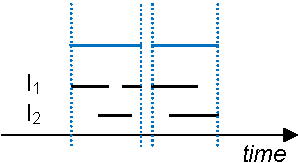
\includegraphics[width=0.31\textwidth]{figures/union}
%\label{fig:cer_replic_times}
}
\subfigure[Intersection.]{
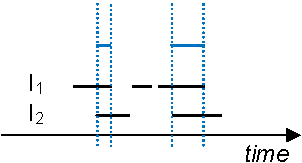
\includegraphics[width=0.31\textwidth]{figures/intersection}
%\label{fig:cer_replic_mem}
}
\subfigure[Relative Complement.]{
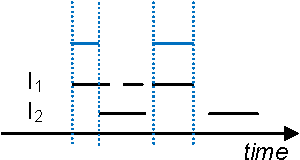
\includegraphics[width=0.31\textwidth]{figures/rcomplement}
%\label{fig:cer_replic_mes}
}
\caption{A visual illustration of the three interval manipulation constructs of RTEC. In this example, there are two input fluent streams, $I_1$ and $I_2$. The output of each interval manipulation construct is colored light blue.}
\label{fig:interval-manipulation}
\end{figure}


In our example, \textttsmall{happy} is a statically determined fluent defined by means of \unionall. 
However, this is just one way of defining happiness. For example, we could have specified that a person is happy when he is rich \textit{and} at the pub. To specify \textttsmall{happy} in this way one should replace \unionall\ by \intersectall\ in the \holdsFor\ rule of \textttsmall{happy}.

The interval manipulation constructs of RTEC support the following type of definition: for all time-points \textttsmall{T}, \textttsmall{F=V} holds at \textttsmall{T} if and only if some Boolean combination of fluent-value pairs holds at \textttsmall{T}. For a wide range of fluents, this is a much more concise definition than the traditional style of Event Calculus representation, i.e.~identifying the various conditions under which the fluent is initiated and terminated so that maximal intervals can then be computed using the domain-independent \holdsFor. Compare, e.g.~the statically determined fluent representation of \textttsmall{happy} in Listing~\ref{lst:rules} and the simple fluent representation below:

{\small
\begin{verbatim}
initiatedAt(happy(X)=true, T) :- 
    initiatedAt(rich(X)=true, T).
initiatedAt(happy(X)=true, T) :-
    initiatedAt(loc(X)=pub, T).
terminatedAt(happy(X)=true, T) :-
    terminatedAt(rich(X)=true, T)
    not holdsAt(loc(X)=pub, T).
terminatedAt(happy(X)=true, T) :-
    terminatedAt(loc(X)=pub, T),
    not holdsAt(rich(X)=true, T).
\end{verbatim}
}

\textttsmall{not} is negation by failure. The interval manipulation constructs of RTEC can also lead to much more efficient computation \cite{DBLP:journals/tkde/ArtikisSP15}.

\subsection{Declarations}\label{sec:declarations}

The declarations of our example were presented in Listing \ref{lst:declarations}.
In the declarations of an event description, we first need to denote the events, simple fluents and statically determined fluents. This is done with the use of the \textttsmall{event},  \textttsmall{simpleFluent} and \textttsmall{sDFluent} predicates.

%\subsubsection{Input Entities, Output Entities \& Indexing}

Each event and fluent must be declared as either \textttsmall{inputEntity} or \textttsmall{outputEntity}. As explained earlier in the section, the input entities may consist of events and/or statically determined fluents, while the output entities may comprise events, simple and/or statically determined fluents.

For each event and fluent, the user must also declare its \textttsmall{index}. In our example, \textttsmall{Person} is the index of all events and fluents. The index allows for the fast retrieval from the memory of the list of time-points, in the case of events, and maximal intervals, in the case of fluents. 

%\subsubsection{Grounding}

To perform query computation, RTEC grounds every output entity. This process is guided by the \textttsmall{grounding} predicate of the declarations language of RTEC, that denotes the domain of the variables of the output entities.  

%\subsubsection{Caching Order}

The final step in the declarations is to specify the \textttsmall{cachingOrder}, i.e.~the order in which the output entities will be processed. To take advantage of RTEC's caching technique, the output entities should be processed in a bottom-up manner. This way, when processing an output entity \textttsmall{U} of level $n$, the time-points/intervals of all entities defining \textttsmall{U}---these will all be in levels below $n$--- will simply be retrieved from the cache. 

Back to our example, if we look the rules, we will see that \textttsmall{happy} is defined in terms of \textttsmall{location} and \textttsmall{rich}. Thus, \textttsmall{location} and \textttsmall{rich} must must be processed before \textttsmall{happy}. \textttsmall{location} and \textttsmall{rich} are on the same level of the hierarchy and thus the order in which they are processed does not matter.


\section{Reasoning in RTEC}\label{sec:reasoning example}

Reasoning has to be efficient enough to support real-time decision-making, and scale to very large numbers of input and output entities. Input entities may not necessarily arrive at RTEC in a timely manner, i.e.~there may be a (variable) delay between the time at which input entities take place and the time at which they arrive at RTEC. Moreover, input entities may be revised, or even completely discarded in the future, as in the case where the parameters of an input entity were originally computed erroneously and are subsequently revised, or in the case of retraction of an input entity that was reported by mistake, and the mistake was realised later.

RTEC performs narrative assimilation by computing and storing the maximal intervals of output entities, i.e.~the intervals of fluents and the time-points in which events occur. Reasoning takes place at specified query times $Q_1, Q_{2}, \dots$. At each $Q_i$ the input entities that fall within a specified interval --- the window $\omega$ --- are taken into consideration. All input entities that took place before or at $Q_i{-}\omega$ are discarded. This is to make the cost of reasoning dependent only on $\omega$ and not on the complete history. The size of $\omega$ and the temporal distance between two consecutive query times --- the slide step $Q_{i}{-}Q_{i-1}$ --- are set by the user. 

At $Q_i$, the output entity maximal intervals computed by RTEC are those that can be derived from the input entities that occurred in the interval $(Q_{i}{-}\omega, Q_{i}]$, as recorded at time $Q_i$. When $\omega$ is longer than the slide step, i.e., when $Q_{i}{-}\omega {<} Q_{i-1} {<} Q_{i}$, it is possible that an input entity occurs in the interval $(Q_{i}{-}\omega, Q_{i-1}]$ but arrives at RTEC only after $Q_{i-1}$; its effects are taken into account at query time $Q_i$. And similarly for input entities that took place in $(Q_{i}{-}\omega, Q_{i-1}]$ and were subsequently revised after $Q_{i-1}$. In the common case that input entities arrive at RTEC with delays, or there is input entity revision, it is preferable therefore to make $\omega$ longer than the slide step. 
Note that information may still be lost. Any input entities arriving or revised between $Q_{i-1}$ and $Q_i$ are discarded at $Q_i$ if they took place before or at $Q_i{-}\omega$. 
To reduce the possibility of losing information, one may increase the size of $\omega$. Doing so, however, decreases recognition efficiency. In what follows we give an example and a detailed account of the `windowing' algorithm of RTEC.

\begin{figure}[t]
	\centering
		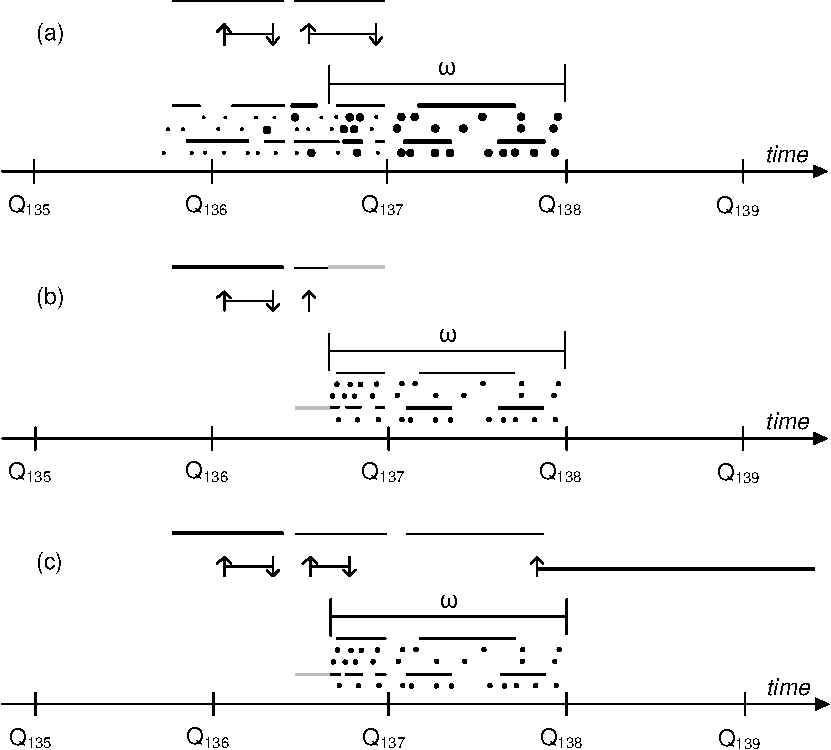
\includegraphics[width=0.6\textwidth]{figures/caching-EC}
	\caption{Windowing in RTEC.}
	\label{fig:rtec-abc}
\end{figure}

Figure \ref{fig:rtec-abc} illustrates windowing in RTEC. In this example we have  $\omega{>}Q_i{-}Q_{i-1}$. To avoid clutter, Figure \ref{fig:rtec-abc} shows streams of only five input entities. These are displayed below $\omega$, with dots for instantaneous input entities and lines for durative ones. For the sake of the example, we are interested in just two fluents:
%
\begin{itemize}
 \item A simple fluent \textttsmall{Se}. The maximal intervals of \textttsmall{Se} are displayed above $\omega$ in Figure \ref{fig:rtec-abc}.
 
 \item A statically determined fluent \textttsmall{Std}. For the example, the maximal intervals of \textttsmall{Std} are defined to be the union of the maximal intervals of the two durative input entities in Figure \ref{fig:rtec-abc}.  The maximal intervals of \textttsmall{Std} are displayed above the \textttsmall{Se} intervals.
\end{itemize}
%
For simplicity, we assume that both \textttsmall{Se} and \textttsmall{Std} are defined only in terms of input entities, i.e.~they are not defined in terms of other output entities.

Figure \ref{fig:rtec-abc} shows the steps that are followed at an arbitrary query time, say $Q_{138}$. Figure \ref{fig:rtec-abc}(a) shows the state of RTEC as computation begins at $Q_{138}$. All input entities that took place before or at $Q_{137}{-}\omega$ were retracted at $Q_{137}$. The thick lines and dots represent the input entities that arrived at RTEC between $Q_{137}$ and $Q_{138}$; some of them took place before $Q_{137}$. Figure \ref{fig:rtec-abc}(a) also shows the maximal intervals for the fluents \textttsmall{Se} and \textttsmall{Std} that were computed and stored at $Q_{137}$.

Reasoning at $Q_{138}$ considers the input entities that took place in $(Q_{138}{-}\omega, Q_{138}]$. All input entities that took place before or at $Q_{138}{-}\omega$ are discarded, as shown in Figure \ref{fig:rtec-abc}(b). For durative input entities that started before $Q_{138}{-}\omega$ and ended after that time, RTEC retracts the sub-interval up to and including $Q_{138}{-}\omega$. Figure \ref{fig:rtec-abc}(b) shows the interval of an input entity that is partially retracted in this way. 

Now consider output entity intervals. At $Q_i$ some of the maximal intervals computed at $Q_{i-1}$ might have become invalid. This is because some input entities occurring in $(Q_i{-}\omega, Q_{i-1}]$ might have arrived or been revised after $Q_{i-1}$: their existence could not have been known at $Q_{i-1}$. Determining which output entity intervals should be (partly) retracted in these circumstances can be computationally very expensive \cite{DBLP:journals/tkde/ArtikisSP15}. We find it simpler, and more efficient, to discard all output entity intervals in $(Q_i{-}\omega, Q_i]$ and compute all intervals from scratch in that period. Output entity intervals that have ended before or at $Q_i{-}\omega$ are discarded. Depending on the user requirements, these intervals may be stored in a database for retrospective inspection of the activities of a system.

In Figure~\ref{fig:rtec-abc}(b), the earlier of the two maximal intervals computed for \textttsmall{Std} at $Q_{137}$ is discarded at $Q_{138}$ since its endpoint is before $Q_{138}{-}\omega$. The later of the two intervals overlaps $Q_{138}{-}\omega$ (an interval `overlaps' a time-point $t$ if the interval starts before or at $t$ and ends after or at that time) and is partly retracted at $Q_{138}$. Its starting point could not have been affected by input entities arriving between $Q_{138}{-}\omega$ and $Q_{138}$ but its endpoint has to be recalculated. Accordingly, the sub-interval from $Q_{138}{-}\omega$ is retracted at $Q_{138}$.

In this example, the maximal intervals of \textttsmall{Std} are determined by computing the union of the maximal intervals of the two durative input entities shown in Figure \ref{fig:rtec-abc}. At $Q_{138}$, only the input entity intervals in $(Q_{138}{-}\omega, Q_{138}]$ are considered. In the example, there are two maximal intervals for \textttsmall{Std} in this period as can be seen in Figure~\ref{fig:rtec-abc}(c). The earlier of them has its start-point at $Q_{138}{-}\omega$. Since that abuts the existing, partially retracted sub-interval for \textttsmall{Std} whose endpoint is $Q_{138}{-}\omega$, those two intervals are amalgamated into one continuous maximal interval as shown in Figure~\ref{fig:rtec-abc}(c). In this way, the endpoint of the \textttsmall{Std} interval that overlapped $Q_{138}{-}\omega$ at $Q_{137}$ is recomputed to take account of input entities available at $Q_{138}$. (In this particular example, it happens that the endpoint of this interval is the same as that computed at $Q_{137}$. That is merely a feature of this particular example. Had \textttsmall{Std} been defined e.g.~as the \emph{intersection} of the maximal intervals of the two durative input entities, then the intervals of \textttsmall{Std} would have changed in $(Q_{138}{-}\omega, Q_{137}]$.)
 

Figure \ref{fig:rtec-abc} also shows how the intervals of the simple fluent \textttsmall{Se} are computed at $Q_{138}$. Arrows facing upwards (downwards) denote the starting (ending) points of the intervals of \textttsmall{Se}. 
First, in analogy with the treatment of statically determined fluents, the earlier of the two \textttsmall{Se}   intervals in Figure~\ref{fig:rtec-abc}(a), and its start and endpoints, are retracted. They occur before $Q_{138}{-}\omega$. The later of the two intervals overlaps $Q_{138}{-}\omega$. The interval is retracted, and only its starting point is kept; its new endpoint, if any, will be recomputed at $Q_{138}$. See Figure \ref{fig:rtec-abc}(b). For simple fluents, it is simpler, and more efficient, to retract such intervals completely and reconstruct them later from their start and endpoints by means of the domain-independent \holdsFor\ rules, rather than keeping the sub-interval that takes place before $Q_{138}{-}\omega$, and possibly amalgamating it later with another interval, as we do for statically determined fluents.
%
%If the last, or any other interval of \textttsmall{Se} that was computed at $Q_{137}$, had started after $Q_{138}{-}\omega$, then the interval and its starting point (and ending point) would have been discarded when the CE recognition process commenced at $Q_{138}$. 
%All ending points after $Q_{138}{-}\omega$, computed at $Q_{137}$, are also discarded.
%

The second step for \textttsmall{Se} at $Q_{138}$ is to calculate its starting and ending points by evaluating the relevant \initiatedAt\ and \terminatedAt\ rules. For this, we only consider input entities that took place in $(Q_{138}{-}\omega, Q_{138}]$. 
Figure \ref{fig:rtec-abc}(c) shows the starting and ending points of \textttsmall{Se} in $(Q_{138}{-}\omega, Q_{138}]$. The last ending point of \textttsmall{Se} that was computed at $Q_{137}$ was invalidated in the light of the new input entities that became available at $Q_{138}$ (compare Figures \ref{fig:rtec-abc}(c)--(a)). Moreover, another ending point was computed at an earlier time.  

Finally, in order to process \textttsmall{Se} at $Q_{138}$ we use the domain-independent \holdsFor\ to calculate the maximal intervals of \textttsmall{Se} given its starting and ending points. The later of the  two \textttsmall{Se} intervals computed at $Q_{137}$ became shorter when re-computed at $Q_{138}$. The second interval of \textttsmall{Se} at $Q_{138}$ is open: given the input entities available at $Q_{138}$, we say that \textttsmall{Se} holds \emph{since} time $t$, where $t$ is the last starting point of \textttsmall{Se}.

The example used for illustration shows how RTEC performs reasoning. In the following section we have a closer look at the operation of RTEC, discussing each of its modules.



% This section is mainly about reasoning
\section{Operation of RTEC}\label{sec:architecture}

Figure \ref{fig:rtec-main} illustrates the architecture of RTEC. In this section, we examine the modules of this architecture.

\begin{figure}[t]
	\centering
		\makebox[\textwidth][c]{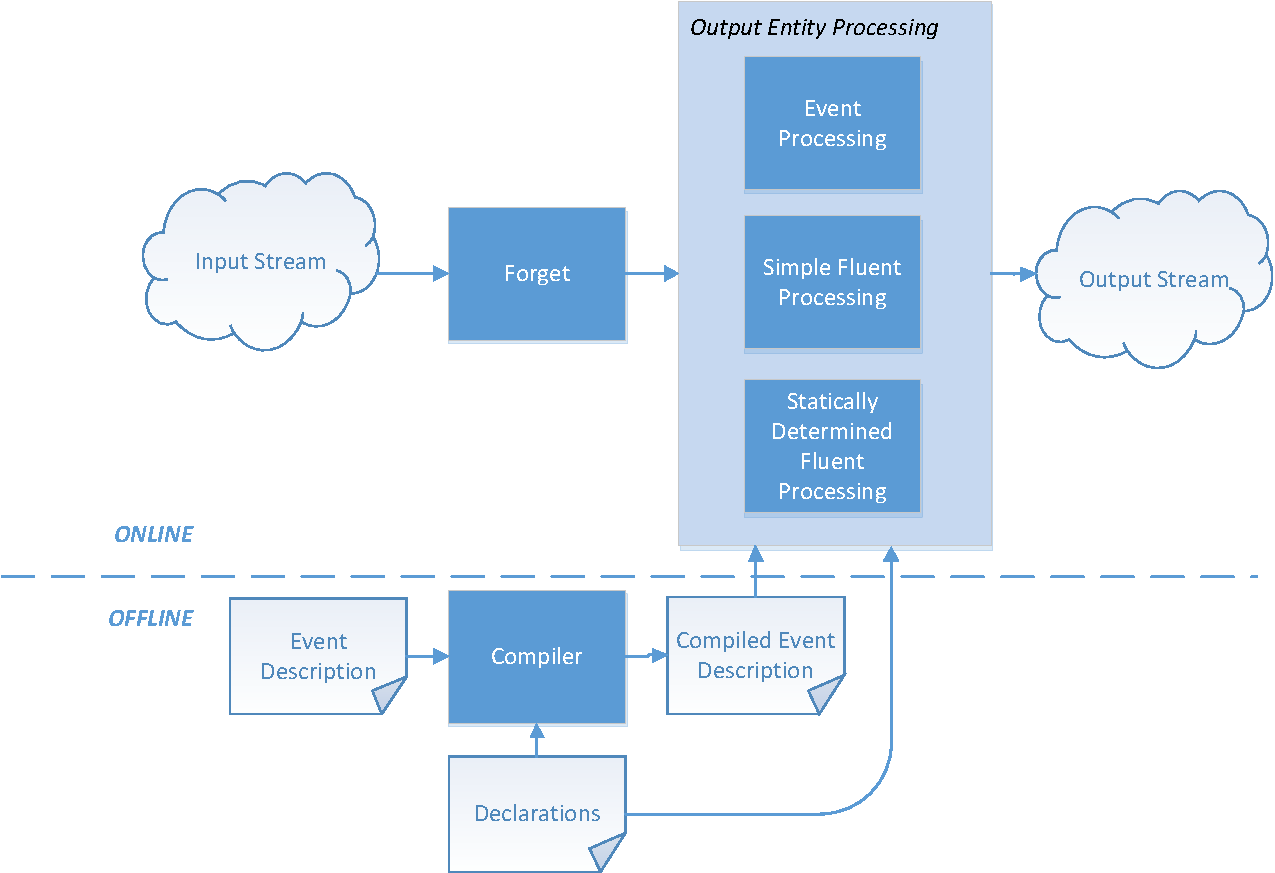
\includegraphics[width=0.8\textwidth]{figures/RTEC_diagram}}
	\caption{The architecture of RTEC.}
	\label{fig:rtec-main}
\end{figure}

\subsection{Offline Activities}\label{sec:compilation}

Before the commencement of online activities, RTEC compiles the event description into a format that allows for more efficient reasoning. This is an offline process which is transparent to the user. 
%
The compiler is called via the predicate: 

{\small
\begin{verbatim}
   ?- compileEventDescription(+Declarations, +EventDecription, 
                              -CompiledEventDescription).
\end{verbatim}
}

The input of this predicate is the event description file (such as Listing \ref{lst:rules}) and the declarations file (e.g.~Listing \ref{lst:declarations}). The output of this predicate is the compiled event description file which is subsequently used for online reasoning --- see the bottom part (`offline') of Figure \ref{fig:rtec-main}.

The aim of the compilation is to eliminate the number of unsuccessful evaluations of \happensAt, \holdsFor\ and \holdsAt, and to introduce additional indexing information.
These atoms are rewritten using specialised predicates, depending on whether they appear in the head or the body of a rule, whether they concern a simple or a statically determined fluent, and whether they host an input or an output entity.

When a \happensAt\ predicate appears in the head of a rule in the Event Description, it is converted into \happensAtEv. On the other hand, \happensAt\ predicates that appear in the body of a rule are converted into \happensAtIE\ (for events that are input entities) or \happensAtProcessed\ (for events that are output entities).

Similarly, the \holdsFor\ predicates appearing in the head of a domain-dependent rule, i.e.~a rule for computing the maximal intervals of statically determined fluents, are rewritten using the predicate \holdsForSDFluent. \holdsFor\ predicates appearing in the body of a rule are translated into \holdsForProcessedSimpleFluent, \holdsForProcessedIE\ or \holdsForProcessedSDFluent\ predicates, according to the fluent type they concern: simple fluents, input (statically determined) fluents, and output statically determined fluents, respectively.

In contrast to the \happensAt\ and \holdsFor\ predicates, \holdsAt\ does not appear in the head of a rule. However, it may appear in the body of \initiatedAt\ and \terminatedAt\ rules; in the case of a simple fluent, the body \holdsAt\ predicate is converted to a \holdsAtProcessedSimpleFluent, whereas in the case of input or output statically determined fluent, it is converted into a \holdsAtProcessedIE\ or a \holdsAtProcessedSDFluent, respectively.

\begin{comment}
\begin{algorithm}[h]                   
\caption{\textttsmall{rtec(}$\mathit{Q_i,\ \omega}$\textttsmall{)} $\qquad\qquad\qquad\qquad\qquad\qquad\qquad\qquad\qquad\qquad\qquad\qquad\qquad\qquad\quad$   
{\small \textbf{Input: }\textttsmall{k}: Depth of hierarchical event description;\ \textttsmall{SimpleFluents(n)}: simple fluents of level \textttsmall{n}; \textttsmall{StdFluents(n)}: statically determined fluents of level \textttsmall{n};\ \textttsmall{Events(n)}: events of level \textttsmall{n}} }
\label{pc:main-RTEC}                          
\begin{algorithmic}[1]
\STATE \textttsmall{forget}$\mathit{( Q_i{-}\omega )}$
%\STATE cachingOrder2(Index,OE)
%\STATE (
%\STATE 
\FOR{\textttsmall{n:=1; n=<k; n++}}
\FORALL{\textttsmall{Std} $\in$ \textttsmall{StdFluents(n)}}  
  \STATE \textttsmall{processSDFluent(Std, }$\mathit{Q_i{-}\omega}$\textttsmall{)}
\ENDFOR
\FORALL{\textttsmall{Se} $\in$ \textttsmall{SimpleFluents(n)}}  
  \STATE \textttsmall{processSimpleFluent(Se, }$\mathit{Q_i{-}\omega}$\textttsmall{)}
\ENDFOR
\FORALL{\textttsmall{Ev} $\in$ \textttsmall{Events(n)}} %\textbf{then} 
  \STATE \textttsmall{processEvent(Ev, }$\mathit{Q_i{-}\omega}$\textttsmall{)}
\ENDFOR
\ENDFOR
\end{algorithmic}
\end{algorithm}
\end{comment}

\subsection{Online Activities}

%Algorithm \ref{pc:main-RTEC} shows the pseudo-code of the main loop of RTEC. 
As already mentioned, reasoning is performed by means of continuous query processing, and concerns the computation of the maximal intervals of output entities, i.e.~the intervals of simple and statically determined fluents, as well as the time-points in which events occur. At each query time $Q_i$, all input entities that took place before or at $Q_i{-}\omega$ are discarded/`forgotten' (see the `forget' box in Figure \ref{fig:rtec-main}).  
Then, RTEC computes and stores the intervals of each output entity (see `output entity processing' in Figure \ref{fig:rtec-main}). Recall that attention is restricted to hierarchical event descriptions. The form of the hierarchy is specified by the event description developer in the declarations using the \textttsmall{cachingOrder} predicate (see Section \ref{sec:declarations}).
%
RTEC adopts a caching technique where the fluents and events of the event description are processed in a bottom-up manner; this way, the intervals (resp.~time-points) of the fluents (events) that are required for the processing of a fluent (event) of level $n$ will simply be fetched from the cache without the need for re-computation. %This technique is illustrated in the outer for-loop of Algorithm \ref{pc:main-RTEC} (see lines 2--12) where fluent (event) processing starts at level 1 of the hierarchical event description and proceeds towards the top (\textttsmall{k}) level. %The fluents (events) of the same level may be processed in any order. For illustration purposes, in Algorithm 1 the following order is adopted: statically determined fluents (lines 4--6), simple fluents (lines 7--9) and events (lines 10--12).
In the following sections we discuss the processes of `forgetting', fluent and event processing. 

\subsubsection{Forget Mechanism}

At each query time $Q_i$, RTEC first discards --- `forgets' --- all input entities that end before or on $\mathit{Q_i{-}\omega}$. For each input entity available at $Q_i$, RTEC:
%
\begin{itemize}
 \item Completely retracts the input entity if the interval attached to it ends before or on $\mathit{Q_i{-}WM}$.
 \item Partly retracts the interval of the input entity if it starts before or on $\mathit{Q_i{-}WM}$ and ends after that time. More precisely, RTEC retracts the input entity interval \textttsmall{(Start,End)} and asserts the interval \textttsmall{(}$\mathit{Q_i{-}\omega}$\textttsmall{,End)}. 
\end{itemize}   

\subsubsection{Statically Determined Fluent Processing}

%The next operation is about looking for intervals in which output Statically Determined Fluents hold. The \textttsmall{processSDFluents} operation follows the same approach as the previous two operations. This time we are looking for \textttsmall{holdsForSDFluent} predicates in the compiled Event description file. In this case, \textttsmall{processSDFluents} will construct this interval from the intervals of the Fluents in the body of the \textttsmall{holdsForSDFluent} clause. To do this, our operation uses ``Interval manipulation'' techniques, in the auxiliary ``Utilities'' module.

After `forgetting' input entities, RTEC computes and stores the intervals of each output entity. At the end of reasoning at each query time $Q_i$, all computed fluent intervals are stored in the computer memory as \simpleFPList\ and \sdFPList\ assertions. \textttsmall{I} in \textttsmall{sdFPList(Index, std, I, PE)} (resp.~\textttsmall{simpleFPList(Index, se, I, PE)}) represents the intervals of statically determined fluent \textttsmall{Std} (simple fluent \textttsmall{Se}) starting in $(Q_{i}{-}\omega, Q_{i}]$, sorted in temporal order. \textttsmall{PE} stores the interval, if any, ending at $Q_{i}{-}\omega$. The first argument in \sdFPList\ (\simpleFPList) is an index that allows for the fast retrieval of stored intervals for a given fluent  even in the presence of very large numbers of fluents. When the user queries  the maximal intervals of a fluent, RTEC amalgamates \textttsmall{PE} with the intervals in \textttsmall{I}, producing a list of maximal intervals ending in $[Q_{i}{-}\omega, Q_{i}]$ and, possibly, an open interval starting in $[Q_{i}{-}\omega, Q_{i}]$.


\begin{algorithm}[h]                   
\caption{ \textttsmall{processSDFluent(Std,}\ $\mathit{Q_i{-}\omega}$\textttsmall{)} }  
\label{pc:recogniseSDFluent}                          
\begin{algorithmic}[1]
\STATE \textttsmall{indexOf(Std, Index)}
\STATE \textttsmall{retract(sdFPList(Index, Std, OldI, OldPE))}
\STATE \textttsmall{amalgamate(OldPE, OldI, OldList)}
\IF {\textttsmall{Start,End:[Start,End)} $\in$ \textttsmall{OldList } $\wedge\ $ \textttsmall{End>}$\mathit{Q_i{-}\omega\ \wedge\ }$ \textttsmall{Start=<} $\mathit{Q_i{-}\omega}$ } %\textbf{then} 
\STATE \textttsmall{PE:=[(Start,}$\mathit{Q_i{-}\omega{+}1}$\textttsmall{)]}
\ELSE 
\STATE \textttsmall{PE:=[]}
\ENDIF 
\STATE \textttsmall{holdsFor(SF, I)}
\STATE \textttsmall{assert(sdFPList(Index, SF, I, PE))}
\end{algorithmic}
\end{algorithm}


Listing \ref{pc:recogniseSDFluent} shows the pseudo-code of \processSDFluent, the procedure for computing and storing the intervals of statically determined fluents. First, RTEC retrieves from \sdFPList\ the maximal intervals of a statically determined fluent \textttsmall{Std} computed at $Q_{i{-}1}$ and checks if there is such an interval that overlaps $Q_i{-}\omega$ (lines 1--8). In Listing~\ref{pc:recogniseSDFluent}, \textttsmall{OldI} represents the intervals of \textttsmall{Std} computed at $Q_{i-1}$. These intervals are temporally sorted and start in $(Q_{i-1}{-}\omega, Q_{i-1}]$. \textttsmall{OldPE} stores the interval, if any, ending at $Q_{i-1}{-}\omega$. RTEC amalgamates \textttsmall{OldPE} with the intervals in \textttsmall{OldI}, producing \textttsmall{OldList} (line 3). If there is an interval  $[$\textttsmall{Start,End}$)$ in \textttsmall{OldList} that overlaps $Q_i{-}\omega$, then the sub-interval $[$\textttsmall{Start,}$\mathit{Q_i{-}\omega{+}1)}$ is retained. See \textttsmall{PE} in Listing \ref{pc:recogniseSDFluent}. All intervals in \textttsmall{OldList} after $Q_i{-}\omega$ are discarded.

At the second step of \processSDFluent, RTEC evaluates \holdsForSDFluent\ rules to compute the \textttsmall{Std} intervals from input entities recorded as occurring in $(Q_i{-}\omega, Q_i]$ (line 9). Prior to the run-time recognition process, RTEC has transformed \holdsFor\ rules concerning statically determined fluents into \holdsForSDFluent\ rules, in order to avoid unnecessary \holdsFor\ rule evaluations (see Section \ref{sec:compilation} for the compilation stage). The intervals of \textttsmall{Std} computed at the previous query time $Q_{i-1}$ are not taken into consideration in the evaluation of \holdsForSDFluent\ rules. The computed list of intervals \textttsmall{I} of \textttsmall{Std}, along with \textttsmall{PE}, are stored in \sdFPList\ (line 10), replacing the intervals computed at $Q_{i-1}$. (Recall that, when the user queries the maximal intervals of a fluent, RTEC amalgamates \textttsmall{PE} with the intervals in \textttsmall{I}.)



\subsubsection{Simple Fluent Processing}

\processSimpleFluent, the procedure for computing and storing simple fluent intervals, also has two parts. First, RTEC checks if there is a maximal interval of the fluent \textttsmall{Se} that overlaps $Q_i{-}\omega$. If there is such an interval then it will be discarded, while its starting point will be kept. 
Second, RTEC computes the starting points of \textttsmall{Se} by evaluating \initiatedAt\ rules, without considering the starting points calculated at $Q_{i-1}$. The starting points are given to \holdsForSimpleFluent, into which \holdsFor\ calls computing the maximal intervals of simple fluents are translated at compile time. This program is defined as follows:

{\small
\begin{verbatim}
holdsForSimpleFluent(SP, Se, I) :- 
     SP <> [],
     computeEndingPoints(Se, EP),
     makeintervals(SP, EP, I).
\end{verbatim}
}

If the list of starting points is empty (first argument of \holdsForSimpleFluent) then the empty list of intervals is returned. Otherwise, \holdsForSimpleFluent\ computes the ending points \textttsmall{EP} of the fluent by evaluating \terminatedAt\ rules, without considering the ending points calculated at $Q_{i-1}$, and then uses \textttsmall{makeIntervals} to compute its maximal intervals given its starting and ending points. 

\begin{figure}[h]
    \centering
    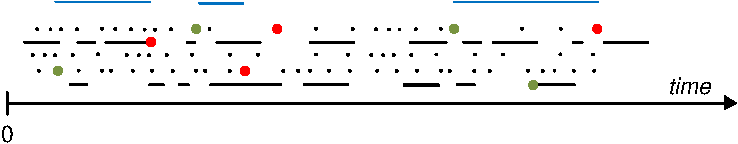
\includegraphics[width=.6\textwidth]{figures/sf4}
    \caption{Maximal interval computation for simple fluents.}
    \label{fig:makeIntervals}
\end{figure}

Figure \ref{fig:makeIntervals} illustrates the process of \textttsmall{makeIntervals}. The black lines and dots indicate streams of durative and instantaneous input entities. The green dots denote starting/initiating points while the red dots indicate ending/terminating points.  
Note that \textttsmall{initiatedAt(F=V, T)} does not necessarily imply that \textttsmall{F<>V} at \textttsmall{T}. Similarly, \textttsmall{terminatedAt(F=V, T)} does not necessarily imply that \textttsmall{F=V} at \textttsmall{T}. 
\textttsmall{makeIntervals} finds all time-points \textttsmall{Ts} at which the fluent \textttsmall{Se} is initiated, and then, for each \textttsmall{Ts}, it computes the first time-point \textttsmall{Tf} after \textttsmall{Ts} at which \textttsmall{Se} is terminated.
Suppose, for example, that  \textttsmall{Se} is initiated at time-points 10 and 20 and terminated at time-points 25 and  30 (and at no other time-points). In that case \textttsmall{Se} holds at all \textttsmall{T} such that 10 $<$ \textttsmall{T} $\leq$ 25. 

\subsubsection{Event Processing}

\textttsmall{processEvents} is the procedure for computing and storing the time-points in which output events occur. In brief, \textttsmall{processEvents} first retracts all computed time-points of the output event in $(Q_{i}-\omega, Q_i]$, and then evaluates \textttsmall{happensAtEv} rules into which domain-dependent \happensAt\ calls are translated at compile time.


\section{Further Information}

The repository of RTEC --- \url{https://github.com/aartikis/RTEC} --- includes event descriptions of application domains, as well as datasets and execution scripts for experimentation. 


%\section{An Integrated Example}

We now present a larger, more realistic use case of RTEC; Performing Event Recognition in order to support city transport management (CTM). The system has been tested in the city of Helsinki, Finland. Buses and trams are equipped with sensors that send GPS coordinates, in-vehicle temperature, noise level and acceleration information to a central server, providing information about the current status of the transport system (for example, the location of buses and trams on the city map). Given the SDE extracted from these sensors, from other data sources such as digital maps, and from the communication between the drivers and the public transport control centre, CE are recognised related to the punctuality of a vehicle, passenger and driver comfort, passenger and driver safety, and passenger satisfaction, among others. The recognised CE are made available to the public transport control centre in order to facilitate decision-making. The choice of CE in this example, and their definitions, were specified by the domain experts (end users).

Short-term activities can be viewed as SDE while long-term activities can be viewed as CE. Consequently, the input to RTEC in this case study includes the set of annotated short-term activities, hereafter SDE, and the output is a set of recognised long-term activities, hereafter CE.

We chose the CTM use case because its CE definitions are fairly complex, allowing us to show many interesting aspects of RTEC. In what follows we present the input to RTEC, a subset of the CE definitions, as well as the data required, and the preparation needed for the Event Recognition.

\subsection{Simple Derived Events \& Composite Events}\label{sec:ctm-input} 

The input to RTEC for the CTM application includes the instantaneous SDE $\mathit{enter\_stop}$, $\mathit{leave\_stop}$, $\mathit{internal\_temperature\_change}$, $\mathit{noise\_level\_change}$ and $\mathit{passenger\_density\_change}$. We represent the instantaneous SDE using the \happensAt\ predicate. For example, the fact \linebreak$\happensAt\mathit{(noise\_level\_change(17, bus, high),\ 415)}$ expresses that the noise level became high in bus $\mathit{17}$ at time-point $\mathit{415}$.

The input to RTEC for CTM also includes durative SDE: $\mathit{abrupt\_acceleration}$, $\mathit{abrupt\_deceleration}$ and $\mathit{sharp\_turn}$. Durative SDE are represented by means of the \holdsFor\ predicate. $\holdsFor\mathit{(abrupt\_acceleration(27, tram)\val very\_abrupt,}$ $\mathit{[(345, 500), (600, 750)])}$, for example, expresses that tram $\mathit{27}$ accelerated `very abruptly' during the intervals $\mathit{[345,500)}$ and $\mathit{[600,750)}$. (Suitable thresholds have been defined by the PRONTO SDE detection system by which it is possible to differentiate between abrupt acceleration and `very' abrupt acceleration, and abrupt deceleration and `very' abrupt deceleration.)

Given the aforementioned SDE, RTEC recognises, among others, the instantaneous $\mathit{punctuality\_change}$ CE, and the durative $\mathit{driving\_style}$, $\mathit{driving\_quality}$, $\mathit{passenger\_comfort}$, $\mathit{driver\_comfort}$ and $\mathit{passenger\_satisfaction}$ CE. Like SDE, the instantaneous CE are represented by means of \happensAt, while the durative ones are represented by \holdsFor.

In the following subsection we present examples of CE definitions.

\subsection{Composite Event Definitions}\label{sec:ctm-definitions} 

% ============== PUNCTUALITY

A vehicle is said to be punctual if it arrives at a stop on or before the scheduled time, and leaves the stop at the scheduled time. A vehicle is said to be non-punctual if it arrives at a stop after the scheduled time, or leaves the stop before or after the scheduled time. $\mathit{enter\_stop}$ and $\mathit{leave\_stop}$ are instantaneous SDE, determined from sensor data and a database of timetable information. The durative $\mathit{punctuality}$ CE is represented as a simple fluent and defined in RTEC as follows:
%
\begin{align}
& \label{eq:ctm-initially-punctuality}
\begin{mysplit}
\initially( punctuality(\_, \_)\val punctual )
\end{mysplit}\\
& \label{eq:ctm-punctuality1}
\begin{mysplit}
\initiatedAt( \mathit{punctuality(Id, VehicleType)\val punctual,\ T} ) \leftarrow \\
\qquad	\happensAt\mathit{( stop\_enter(Id, VehicleType, \_StopCode, scheduled),\ T)}	
\end{mysplit}\\
& \label{eq:ctm-punctuality2}
\begin{mysplit}
\initiatedAt( \mathit{punctuality(Id, VehicleType)=punctual,\ T} ) \leftarrow \\
\qquad	\happensAt\mathit{( stop\_enter(Id, VehicleType, \_StopCode, early),\ T)}
\end{mysplit}\\
& \label{eq:ctm-punctuality3}
\begin{mysplit}
\initiatedAt( \mathit{punctuality(Id, VT)\val non\_punctual,\ T} ) \leftarrow \\
\qquad  \happensAt\mathit{( stop\_enter(Id, VehicleType, \_StopCode , late),\ T )}
\end{mysplit}\\
& \label{eq:ctm-punctuality4}
\begin{mysplit}
\initiatedAt( \mathit{punctuality(Id, VT)\val non\_punctual,\ T} ) \leftarrow \\
\qquad  \happensAt\mathit{( stop\_leave(Id, VehicleType, \_StopCode , early),\ T )}
\end{mysplit}
\end{align}
%
`$\_$' is an `anonymous' Prolog variable. $\mathit{Id}$ is an integer serving as the identifier of a vehicle, while $\mathit{VT}$ represents the vehicle type (tram or bus). The third argument of the $\mathit{enter\_stop}$ and $\mathit{leave\_stop}$ SDE is an integer denoting the code of a bus/tram stop, and the fourth argument expresses whether the vehicle entered/left the stop on, before or after the scheduled time.

Initially, every vehicle is punctual; thereafter $\mathit{punctuality}$ is affected by the $\mathit{enter\_stop}$ and $\mathit{leave\_stop}$ SDE. The maximal intervals during which a vehicle is continuously (non-)punctual are computed from rules \eqref{eq:ctm-initially-punctuality}--\eqref{eq:ctm-punctuality4} by the built-in \holdsFor\ predicate.
%
\begin{align}
& \label{eq:ctm-punctuality5}
\begin{mysplit}
\holdsFor( \mathit{punctuality(Id, VT)\val non\_punctual,\ NPI} ) \leftarrow \\
\qquad \holdsFor( \mathit{punctuality(Id, VT)\val punctual,\ PI} ), \\
\qquad \abscomplementall( [PI], NPI ).
\end{mysplit}
\end{align}
%
This rule uses the domain-independent implementation of \holdsFor\ to compute the maximal intervals for which a vehicle is continuously (non-)punctual. Punctuality change occurs at the first time-point of each of these intervals. There are other, equivalent ways of formulating this definition but since $\mathit{punctuality}$ intervals are to be computed anyway (as required by the end users), this method is the most convenient.

Transport officials are also interested in recognising punctuality \emph{change}.
The following rule expresses the definition of the instantaneous $\mathit{punctuality\_ change}$ CE:
%
\begin{align}
& \label{eq:ctm-punctuality-change1}
\begin{mysplit}
\happensAt( \mathit{punctuality\_change(Id, VehicleType, punctual),\ T} ) \leftarrow \\
\qquad \happensAt( \mathit{end(punctuality(Id, VehicleType)\val non\_punctual),\ T)}
\end{mysplit}\\
& \label{eq:ctm-punctuality-change2}
\begin{mysplit}
\happensAt( \mathit{punctuality\_change(Id, VehicleType, non\_punctual),\ T} ) \leftarrow \\
\qquad	\happensAt( \mathit{end(punctuality(Id, VehicleType)\val unctual),\ T)}
\end{mysplit}
\end{align}
%
Driving style is another aspect that interests city transport officials. Two durative CE concerning driving style are defined as follows:
%
\begin{align}
& \label{eq:ctm-driving-style1}
\begin{mysplit}
\holdsFor( \mathit{driving\_style(Id, VehicleType)=unsafe, UDI} ) \leftarrow \\
\qquad	\holdsFor( \mathit{sharp\_turn(Id, VehicleType)=very\_sharp, VSTI}), \\
\qquad	\holdsFor( \mathit{abrupt\_acceleration(Id, VehicleType)=very\_abrupt, VAAI}), \\
\qquad	\holdsFor( \mathit{abrupt\_deceleration(Id, VehicleType)=very\_abrupt, VADI}), \\
\qquad	\unionall([VSTI, VAAI, VADI], UDI).
\end{mysplit}\\
& \label{eq:ctm-driving-style2}
\begin{mysplit}
\holdsFor( \mathit{driving\_style(Id, VehicleType)=uncomfortable, UDI} ) \leftarrow \\
\qquad	\holdsFor( \mathit{sharp\_turn(Id, VehicleType)=sharp, STI}), \\
\qquad	\holdsFor( \mathit{abrupt\_acceleration(Id, VehicleType)=very\_abrupt, VAAI}), \\
\qquad	\holdsFor( \mathit{abrupt\_deceleration(Id, VehicleType)=very\_abrupt, VADI}),  \\
\qquad	\complementall(STI, [VAAI, VADI], PureSharpTurn), \\
\qquad	\holdsFor( \mathit{abrupt\_acceleration(Id, VehicleType)=abrupt, AAI}), \\
\qquad	\holdsFor( \mathit{abrupt\_deceleration(Id, VehicleType)=abrupt, ADI}), \\
\qquad	\unionall([PureSharpTurn, AAI, ADI], UDI).
\end{mysplit}
\end{align}
%
Rule \eqref{eq:ctm-driving-style1} above defines unsafe driving as the driving that is characterized by very sharp turns and/or very abrupt acceleration/deceleration. Rule \eqref{eq:ctm-driving-style2}, on the other hand defines uncomfortable driving. A driver is considered to be driving uncomfortably if they take sharp turns (but not \textit{very} sharp), and they accelerate/decelerate abruptly (but not \textit{very} abruptly).

\subsection{Event/Fluent Declarations}\label{sec:ctm-declarations}

In subsection \ref{sec:ctm-input} we discussed the Simple, Derived Events, as well as the Composite Events of interest in this use case. In this subsection we will show how these events can be declared in the ``ctm\_declarations.prolog'' file (see also the source code of RTEC).

Based on the CTM rules presented in the previous section, we have 8 input SDEs, of which 2 intantaneous (events $\mathit{stop\_enter/4}$, $\mathit{stop\_leave/4}$) and 6 durative (fluents $\mathit{sharp\_turn/2=sharp}$, $\mathit{sharp\_turn/2=very\_sharp}$, $\mathit{abrupt\_acceleration/2=abrupt}$, $\mathit{abrupt\_acceleration/2=very\_abrupt}$, $\mathit{abrupt\_deceleration/2=abrupt}$, $\mathit{abrupt\_deceleration/2=very\_abrupt}$). We also have 6 Composite Events, of which 2 Events ($\mathit{punctuality\_change(\_,\_,punctual)}$, $\mathit{punctuality\_change(\_,\_,non\_punctual)}$), 2 Simple Fluents ($\mathit{punctuality/2=punctual}$, $\mathit{punctuality/2=non\_punctual}$), and 2 Statically Determined Fluents ($\mathit{driving\_style/2=uncomfortable}$, $\mathit{driving\_style/2=unsafe}$). Table \ref{table:declarations} contains all the above-mentioned entities.
%
\begin{table}
\begin{tabular}{ l | c | c |}
\cline{2-3}
& Input Entities & Output Entities \\ \cline{1-3}
\multicolumn{1}{| l |}{\multirow{2}{*}{Events}} & $\mathit{stop\_enter/4}$ & $\mathit{punctuality\_change(\_,\_,punctual)}$ \\
\multicolumn{1}{| l |}{} & $\mathit{stop\_leave/4}$ & $\mathit{punctuality\_change(\_,\_,non\_punctual)}$ \\ \hline
\multicolumn{1}{| l |}{\multirow{2}{*}{SF}} & & $\mathit{punctuality/2=punctual}$ \\
\multicolumn{1}{| l |}{} & & $\mathit{punctuality/2=non\_punctual}$ \\ \hline
\multicolumn{1}{| l |}{\multirow{6}{*}{SDF}} & $\mathit{sharp\_turn/2=sharp}$ & \\
\multicolumn{1}{| l |}{} & $\mathit{sharp\_turn/2=very\_sharp}$ & $\mathit{driving\_style/2=uncomfortable}$ \\
\multicolumn{1}{| l |}{} & $\mathit{abrupt\_acceleration/2=abrupt}$ & $\mathit{driving\_style/2=unsafe}$ \\
\multicolumn{1}{| l |}{} & $\mathit{abrupt\_acceleration/2=very\_abrupt}$ & \\
\multicolumn{1}{| l |}{} & $\mathit{abrupt\_deceleration/2=abrupt}$ & \\
\multicolumn{1}{| l |}{} & $\mathit{abrupt\_deceleration/2=very\_abrupt}$ & \\
\hline
\end{tabular}
\caption{The entities of the CTM use case}
\label{table:declarations}
\end{table}
%
All these entities are indexed based on the Id of the bus that is involved in them.

Next, we need to state whether the input entities that are SDFs will have their intervals collected into a list or built from time-points. In our case, for each of the input SDFs the intervals are going to be collected into a list. Therefore, we add the following code to the declarations file:
%
\begin{verbatim}
collectIntervals(abrupt_acceleration(_,_)=abrupt).
collectIntervals(abrupt_acceleration(_,_)=very_abrupt).
collectIntervals(abrupt_deceleration(_,_)=abrupt).
collectIntervals(abrupt_deceleration(_,_)=very_abrupt).
collectIntervals(sharp_turn(_,_)=sharp).
collectIntervals(sharp_turn(_,_)=very_sharp).
\end{verbatim}
%
Subsequently, we need to declare the grounding of all the fluents and events that are output entities. We will assign every fluent with a list of possible groundings. All these entities have an arity of 2 and refer to a (vehicle id - vehicle type) pair. Thus, we have built a collection of Prolog facts of the form ``\textttsmall{vehicle(Id, VehicleType).}'' that contains all the vehicles' Ids and types and use this collection to ground the aforementioned entities as follows: 
%
\begin{verbatim}
grounding(abrupt_acceleration(Id,VehicleType)=abrupt) 		:-
        vehicle(Id, VehicleType). 
grounding(abrupt_acceleration(Id,VehicleType)=very_abrupt) 	:-
        vehicle(Id, VehicleType). 
grounding(abrupt_deceleration(Id,VehicleType)=abrupt) 		:-
        vehicle(Id, VehicleType). 
grounding(abrupt_deceleration(Id,VehicleType)=very_abrupt) 	:-
        vehicle(Id, VehicleType). 
grounding(sharp_turn(Id,VehicleType)=sharp) 			:-
        vehicle(Id, VehicleType). 
grounding(sharp_turn(Id,VehicleType)=very_sharp) 		:-
        vehicle(Id, VehicleType).
grounding(punctuality(Id,VehicleType)=punctual) 		:-
        vehicle(Id, VehicleType).   
grounding(punctuality(Id,VehicleType)=non_punctual) 		:-
        vehicle(Id, VehicleType).
grounding(punctuality_change(Id,VehicleType,punctual)) 		:-
        vehicle(Id, VehicleType).
grounding(punctuality_change(Id,VehicleType,non_punctual)) 	:-
        vehicle(Id, VehicleType).
grounding(driving_style(Id,VehicleType)=unsafe) 		:-
        vehicle(Id, VehicleType).
grounding(driving_style(Id,VehicleType)=uncomfortable) 		:-
        vehicle(Id, VehicleType).
\end{verbatim}
%
Finally, we must declare the caching order of the output entities, beginning with the level-1 output entities, that only depend on input (level-0) entities in order to be computed, and forming a hierarchy. In our case, level-1 entities are the Simple Fluents $\mathit{punctuality(\_,\_)=punctual}$ and $\mathit{cachingOrder(punctuality(\_,\_)=non\_punctual)}$, as well as the SDF $\mathit{cachingOrder(driving\_style(\_,\_)=unsafe)}$ and $\mathit{cachingOrder(driving\_style(\_,\_)=uncomfortable)}$, and level-2 entities are the events $\mathit{punctuality\_change(\_,\_,punctual)}$ and $\mathit{punctuality\_change(\_,\_,non_punctual)}$.
%
\begin{verbatim}
cachingOrder(punctuality(_,_)=punctual).    
cachingOrder(punctuality(_,_)=non_punctual).
cachingOrder(driving_style(_,_)=unsafe). 
cachingOrder(driving_style(_,_)=uncomfortable).
cachingOrder(punctuality_change(_,_,punctual)).
cachingOrder(punctuality_change(_,_,non_punctual)).
\end{verbatim}

\subsection{CTM data}\label{sec:ctm-data}

Now that we have analyzed the use case, and have set up our Event Description and Declarations, we must take care of the data we are going to use in order to perform the Event Recognition task. We need 2 tyoes of input data. The event narrative and a collection of facts that forms the background knowledge and concerns the grounding of the fluents and the events that are output entities (see subsection \ref{sec:ctm-declarations}).

The event narrative is stored in a series of assertions. We take the input entities shown in Table \ref{table:declarations} and assert each of their occurrences under an auxiliary ``\textttsmall{updateSDE/3}'' predicate.
%
\begin{verbatim}
updateSDE( sharp_turn, 0, 1000 ) :-
assert( holdsForIESI( sharp_turn(75, bus)=sharp, (3, 50)) ),
assert( holdsForIESI( sharp_turn(75, bus)=sharp, (88, 130)) ),
assert( holdsForIESI( sharp_turn(76, bus)=very_sharp, (720, 912)) ),
assert( holdsForIESI( sharp_turn(77, bus)=sharp, (959, 999)) ).
\end{verbatim}
%
This event narrative excerpt shows that bus 75 performed a sharp turn from time 3 to time 50 and from time 88 to time 130. In addition, bus 76 takes a very sharp turn from time 720 until 912. Finally, bus 77 makes a sharp turn from time 959 to time 999. We construct similar narratives for all input entities, according to the scenario that we are working on.

The background knowledge is stored in a separate file that, as mentioned in subsection \ref{sec:ctm-declarations} (in the grounding stage), contains Prolog facts of the form ``\textttsmall{vehicle(Id, VehicleType).}'' that depict all the vehicles, along with their type.
%
\begin{verbatim}
vehicle(75, bus).
vehicle(76, bus).
vehicle(77, bus).
\end{verbatim}
%
This background knowledge fragment shows that vehicles 75, 76, and 77 are buses.

\subsection{Compilation}\label{sec:ctm-compilation}

Before we are ready to run RTEC and receive the Event Recognition results, we must compile our event description, according to the rules presented in \ref{sec:compilation}. The result of the compilation is a new file that contains elements from both the event description and the declarations file. The rules are now ready to be read and understood by RTEC, during the Event Recognition process. The command and the output are totally similar to the ones we showed in subsection \ref{sec:aSimpleExample}.

\subsection{Performing Event Recognition}\label{sec:ctm-execution}

We have all the necessary components for the Event Recognition. We just need to prepare the main Prolog script and execute it. Using a text editor, we type the following code:

\lstinputlisting[
	style	= Prolog-cvlas,
	caption	= {mini-ctm-queries.prolog file that contains the main ER script},
	label	= {lst:ctm-queries}
]{listings/mini-ctm-queries.prolog}

The above code first imports all the files described in the previous subsections, then itdefines the ``\textttsmall{performER}'' predicate. The structure of the script is the same as in subsection \ref{sec:aSimpleExample}. This time our main predicate has 2 parameters, the Event Recognition step (the temporal distance between two consecutive queries) and the working memory (the interval in which RTEC will look for events/fluents). We initialise the recognition, load our narrative and execute the event assimilation just as we did in the simple example, in the Introduction. The only difference is that we create a new file named ``outputEntities.txt'' that stores the output entities that were calculated during the Event Assimilation process.

We can start a Prolog session, consult ``mini-ctm-queries.prolog'' and then type ``\textttsmall{performER(60,60)}'' (that is, we ask RTEC to perform the Event Recognition with $Step\val 60$ and $Working Memory\val 60$).

If Prolog replies with a message ending in ``yes'', then the procedure was successful. We can open the ``outputEntities.txt'' file and see the results.

\lstinputlisting[
	style	= Prolog-cvlas,
	caption	= {The output entities},
	label	= {lst:ctm-oe}
]{listings/outputEntities.txt}


%\section{A simplified language}\label{sec:simple-language}

Section \ref{sec:RTEC-language} thoroughly discussed the features of the language of RTEC. In this section we will describe a simplified version of the RTEC language, and the Event Calculus, in general.

So far, in order to address an Event Recognition problem, the RTEC users need to be familiar with Prolog, and often have to take care to use several special, built-in predicates and functions -- e.g.: the interval manipulation constructs -- correctly. Another, simpler form of the Event Calculus, with its own compiler has been designed and developed. This simplified Event Calculus (SimplEC) aims at producing much simpler and readable Event Descriptions, even for demanding domains, and at the same time it maintains most of the expressiveness of RTEC.

The time model remains linear, with integer time points. What changes is the representation of the events and fluents, as well as the format of the rules within an Event Description.

First of all, SimplEC is not Prolog, in contrast with the classic RTEC event patterns. It is designed to resemble simple statements in English, with some pseudocode and mathematical elements. It does not contain obscure symbols like \texttt{:-}, or \texttt{\textbackslash +}. Instead, it contains simple words like \texttt{if}, \texttt{or}, \texttt{not}, as well as the comma operator that indicates conjunction. There are also a few special tokens, like \texttt{happens} that stem from the classic RTEC language.

\subsection{Representing events and fluents}

In this simplified version of the RTEC language, there are no special predicates like \texttt{holdsAt(F=V,T)}, \texttt{holdsFor(F=V, I)}, or \texttt{happensAt(E, T)} that indicate happening, holding, initiation and termination, as we have seen on the section about RTEC. All events and fluents are represented using a compound term of the form
%
\begin{align}
& \label{eq:compound_term}
\begin{mysplit}
\mathrm{functor}( \dots \mathit{arguments}\dots )[\val\mathit{value}]
\end{mysplit}
\end{align}
%
where square brackets denote the optional part of the term. This structure allows for the representation of both events and fluents. Specifically, when this term contains a value, then it is always a fluent. When the value is absent, it may either be a fluent with the default ``\texttt{true}'' value, or an event which, by definition, has no value. The distinction between the latter two categories is based on the context.

\subsubsection{Built-in tokens}

There are a handful of built-in keywords that precede the compound terms shown in \ref{eq:compound_term} and help identify how the term is being used. These keywords are:
\begin{itemize}
\item \texttt{initiate}: Indicates that the following term is a fluent and is being initiated. Similar to classic RTEC's $\initiatedAt$.
\item \texttt{terminate}: Indicates that the following term is a fluent and is being terminated. Similar to classic RTEC's $\terminatedAt$.
\item \texttt{start}: Denotes the point in time where the following fluent starts holding. Similar to classic RTEC's $\startE$.
\item \texttt{end}: Denotes the point in time where the following fluent ceases holding. Similar to classic RTEC's $\endE$.
\item \texttt{happens}: Indicates that the following term is an event and expresses its happening. Similar to classic RTEC's $\happensAt$.
\end{itemize}

\subsubsection{Defining simple fluents}

The SimplEC user can state initiation conditions for simple fluents as follows:
%
\begin{align}
& \label{eq:simple_fluent}
\begin{mysplit}
\mathbf{initiate}\ F_1\ \mathbf{if} \\
\qquad E[, \\
\qquad \mathrm{condition}]^*.
\end{mysplit}
\end{align}
%
Termination conditions are structured in the same way, the only difference being that instead of the keyword $\mathbf{initiate}$ we use the keyword $\mathbf{terminate}$.

$F_1$ is a fluent, following the syntax we have seen in \eqref{eq:compound_term}. $E$ can be either an ordinary event structured as in \eqref{eq:compound_term}, or one of the two special events ($\mathbf{start}\ F_2$, $\mathbf{end}\ F_2$), denoting the starting and ending points of the holding interval of another fluent $F_2$, respectively.

$[,\ \mathrm{condition}]^*$ denotes an optional set of conditions surrounding the happening of $E$, that are significant for the initiation or termination of $F_1$. Such a condition could be one of the following:
%
\begin{itemize}
\item $F_3$, meaning that fluent $F_3$ must hold at that specific timepoint.
\item $\mathbf{start}\ F_3$, meaning that $F_3$ must start holding.
\item $\mathbf{end}\ F_3$, meaning that $F_3$ must cease holding.
\item $\mathbf{not}\ F_3$, meaning that $F_3$ must not hold.
\item $\mathbf{happens}\ E_2$, indicating the happening of event $E_2$.
\item $\mathbf{not\ happens}\ E_2$, indicating the absense of event $E_2$.
\item atemporal constraint.
\end{itemize}

In the same fashion that we define the initiation and termination points of a simple fluent, we can also define the happening of events that are output entities. This can be achieved by replacing the $\mathbf{initiate}$ and $\mathbf{terminate}$ keywords with the $\mathbf{happens}$ keyword and putting an event instead of a fluent at the head of the statement. The body of the statement is structured exactly as in the initiation/termination case.

\subsubsection{Defining statically determined fluents}

A SimplEC statement defining a statically determined fluent consists of conjunctions, disjunctions and negations of other fluents, possibly nested within each other. The keyword $\mathbf{or}$ is used in disjunctions, the keyword $\mathbf{not}$ is used in negations, and conjunctions use the comma operator. There are no interval manipulation constructs, as the relevant information is contained in the occurrence of the respective operators and keywords.

The following example shows the definition of moving as a statically determined fluent. Two persons are considered to be moving together while they are both walking and they appear close to each other. This can be expressed in SimplEC as follows:
%
\begin{align}
& \label{eq:move-simplEC}
\begin{mysplit}
\mathit{moving(P_1, P_2)}\ \mathbf{if} \\
\qquad \mathit{walking(P_1),} \\
\qquad \mathit{walking(P_2),} \\
\qquad \mathit{close(P_1, P_2).}\\
\end{mysplit}
\end{align}

Another, more involved example is the definition of fighting. Fighting between two persons takes place when at least one of them is moving abruptly, none of them is totally inactive, and at the same time they are very close to each other. In SimplEC, we write:
%
\begin{align}
& \label{eq:fight-simplEC}
\begin{mysplit}
\mathit{fighting(P_1, P_2)}\ \mathbf{if}\\
\qquad \mathit{(abrupt(P_1)}\ \mathbf{or}\ \mathit{abrupt(P_2))},\\
\qquad \mathit{close(P_1, P_2)},\\
\qquad \mathbf{not}\ \mathit{(inactive(P_1)}\ \mathbf{or}\ \mathit{inactive(P_2))}.
\end{mysplit}
\end{align}

\subsection{Event Description}

An Event Description in SimplEC is a set of statements that follow the above-mentioned syntax. Let's consider a sample Event Description that only contains statements \eqref{eq:move-simplEC} and \eqref{eq:fight-simplEC}. It would look like this:

\begin{minipage}{\linewidth}
\lstinputlisting[
  style      = Prolog-cvlas,
  caption    = {Event description in SimplEC.},
  label	     = {lst:simplec-rules}
]{listings/simplec_rules.txt}
\end{minipage}

This set of rules translates into the following RTEC Event Description:

\begin{minipage}{\linewidth}
\lstinputlisting[
  style      = Prolog-cvlas,
  caption    = {Event description of Listing \ref{lst:simplec-rules} translated into RTEC.},
  label	     = {lst:rtec-rules}
]{listings/rtec_rules.txt}
\end{minipage}

\subsection{Declarations and Dependencies}

The compiler of SimplEC parses a set of statements in the simple language and, based on its grammar, translates the statements to rules in the RTEC format. Moreover, it constructs the declarations required for computing narrative assimilation queries. The declarations distinguish, for the benefit of RTEC, between simple and statically determined fluents, and between input and output entities (events and fluents). 
%The compiler parses each SimplEC statement and identifies each of the entities involved as an event, a simple fluent or a statically determined fluent, as well as deciding whether it is an input or an output entity. 
In SimplEC statement \eqref{eq:move-simplEC}, for instance, the compiler will detect three statically determined fluents, namely $\mathit{moving(\_,\_)}$, $\mathit{walking(\_)}$, and $\mathit{close(\_,\_)}$, of which $\mathit{moving(\_,\_)}$ is an output entity, as it appears in the head of the statement, and the other two are input entities, as they do not appear to be defined by other, simpler entities. This knowledge of the compiler is summarized in the following set of declarations:
%
\begin{align}
& \label{eq:move-decls}
\begin{mysplit}
\mathit{\textsf{\footnotesize sDFluent}(moving(\_, \_)).} \\
\mathit{\textsf{\footnotesize sDFluent}(walking(\_)).} \\
\mathit{\textsf{\footnotesize sDFluent}(close(\_, \_)).}\\
\mathit{\textsf{\footnotesize outputEntity}(moving(\_, \_)).} \\
\mathit{\textsf{\footnotesize inputEntity}(walking(\_)).} \\
\mathit{\textsf{\footnotesize inputEntity}(close(\_, \_)).}\\
\end{mysplit}
\end{align}

\begin{figure*}[t]
\centering
	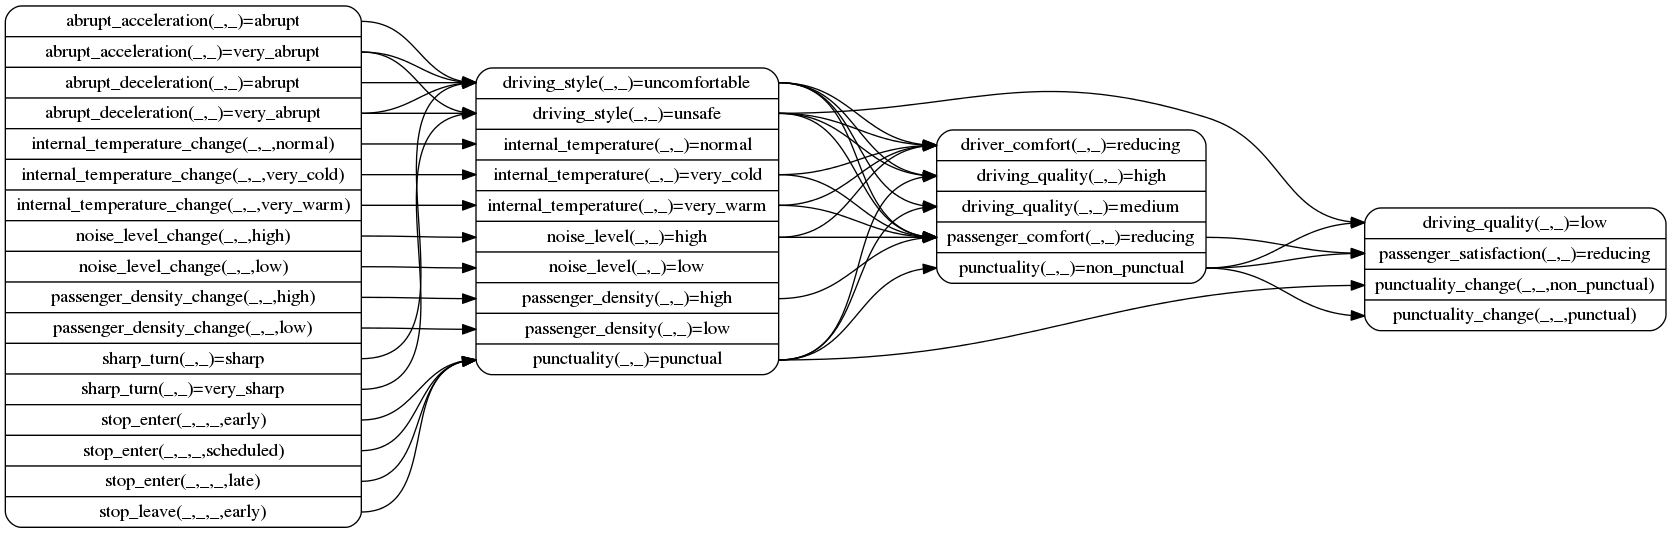
\includegraphics[width=\textwidth]{figures/ctm_graph.png}
	\caption{Dependency graph of the city transport management event description.}
	\label{fig:ctm_graph}
\end{figure*}

The declarations also express the `caching hierarchy', that is, the order in which fluents and events are processed. RTEC performs bottom-up processing whereby fluents and events of level 1 of a hierarchy are processed first, subsequently moving to levels 2, 3, etc. The computed intervals of each level are cached. This way, fluent and event intervals of some level $n$ may be simply fetched from memory when required in the processing of fluents and events of some higher level $m$.

To aid the user, the compiler may display the dependency graph of the event description. This is a directed graph where each vertex corresponds to a fluent or event, and for each pair of vertices $(i, j)$ there is an edge from $i$ to $j$ if $i$ appears in the body of a statement defining $j$. Figure \ref{fig:ctm_graph} shows the dependency graph of an event description for city transport management. In this figure, we can observe the way in which the events and fluents affect each other. In the leftmost part of the figure there are vertices with no incoming edges. These correspond to input events and fluents that form the narrative upon which all complex activities will be recognised. In this domain, the input entities include information about the acceleration and deceleration of  transport vehicles, changes in  internal temperature, noise level or passenger density, as well as the time of arrival at a stop.

On the right of the bottom layer, there are two other layers of events and fluents that have both incoming and outgoing edges. These are output entities that also contribute to the definition of other output entities. On these layers we combine information from the bottom layer and produce higher-level information. For instance, we can recognise complex activities such as driving style and quality, vehicle punctuality and the passengers' comfort level.
In the rightmost part of the figure, there is one last layer with no outgoing edges. These are the complex activities of the highest level---consider, for instance, passenger satisfaction.

\subsection{Running the compiler}

The compiler of the SimplEC language is written in Prolog and is based on Prolog's Definite Clause Grammars, which are often used for NLP purposes and building parsers, in general.

In order to use the compiler, the user must type:
{\small
\begin{verbatim}
   $ swipl -l simplEC.prolog
\end{verbatim}
}

And then, supposing that the user has written their set of SimplEC statements in a file named ``simplec\_rules.txt'', type:
{\small
\begin{verbatim}
   ?- simplEC('simplec_rules.txt', 'event_description.prolog',
                              'declarations.prolog', 'dependency_graph.txt').
\end{verbatim}
}
This will take the file with the event patterns in SimplEC and translate it to an Event description in the classic RTEC format, along with its respective declarations, as we have seen in detail, earlier in this manual. But before the Event Recognition process is started, the rules must be further compiled by the compiler of RTEC this time.

To save time and to unify the two compilation steps, there is an executable script named ``compile.sh'' that calls both compilers and produces the compiled event description and the declarations that are needed for RTEC to start performing Event Recognition. To call that script, the user should write in a command window:
{\small
\begin{verbatim}
   $ bash compile.sh simplec_rules.txt
\end{verbatim}
}


\bibliographystyle{plain}               % basic style, author-year citations
\bibliography{RTEC_manual}

\nocite{*}

\end{document}